\chapter{Online-Algorithmen}

\begin{tcolorbox}[colframe=black!3!white]
  \textbf{Inhalt dieses Kapitels}:
  \tcblower{} 
  \begin{itemize}
    \item Einführung in Online-Algorithmen
    \item Beispiel: Job-Scheduling
    \item Beispiel: Skiausleihe
    \item Beispiel: Speicherverwaltung
    \item Beispiel: Auswahl von Experten
  \end{itemize}
\end{tcolorbox}

\term{Online-Algorithmen}\index{Online-Algorithmus} werden verwendet, wenn Eingabegrößen nicht im Vornerein bekannt sind. Viele Algorithmen, die wir bisher diskutiert haben, benötigen Vorarbeitszeit, um optimale Ergebnisse liefern zu können, und sind daher nicht auf Probleme anwendbar, wo die Eingabe in serieller Natur vorliegt. Die bisher diskutierten Algorithmen werden daher auch \term{Offline-Algorithmen}\index{Offline-Algorithmus} genannt.

\section{Übersicht}

Wir werden uns im Folgenden Konzepte von Online-Algorithmen anhand von Beispielen anschauen. Zuerst definieren wir, was ein Online-Algorithmus formal ist.

\begin{itemize}
  \item \textbf{Eingabe}: Folge von Anforderungen (\emph{requests})
  \begin{equation*}
    \sigma = \left( r_1,\dots, r_n \right) \in R^n
  \end{equation*}
  \item \( r_i \) muss auf Anforderung bearbeitet werden, es entsteht eine Antwort
  \begin{equation*}
    a_i = g_i(r_1, \dots,r_i) \in A\text{.}
  \end{equation*}
  Es sind keine Informationen über die Zukunft verfügbar (\( r_{i+1},\dots \)). Antworten sind unwiderruflich.

  Der konkrete Algorithmus ist also durch \( g_1,\dots \) eindeutig festgelegt.

  \item \textbf{Kosten} \( \text{cost}_n : R^n \times A^n \to \R_{> 0} \)

  \item \textbf{Ausgabe} für \( \sigma \in R^n \) ist also
  \begin{equation*}
    \textsc{alg}[\sigma] = \left( g_1(r_1),g_2(r_1,r_2),\dots,g_n(r_1,\dots,r_n) \right) \in A^n
  \end{equation*}
  und die Kosten
  \begin{equation*}
    \textsc{alg}(\sigma) = \text{cost}_n(\sigma,\textsc{alg}[\sigma])
  \end{equation*}
\end{itemize}

\subsection{Kompetitive Analyse}

Um einschätzen zu können, wie gut ein Online-Algorithmus ist, vergleichen wir ihn mit einem optimalen Offline-Algorithmus --- das ist die \term{Kompetitive Analyse}\index{Kompetitive Analyse} dieses Online-Algorithmus.

\begin{definition}[c-kompetitiv]
  Ein Online-Algorithmus ist für ein Optimierungsproblem auf Input \( \sigma \) \term{\( c \)-kompetitiv}\index{kompetitiv!c}, falls es einen Offline-Algorithmus OPT gibt, der nach einem Kostenmaß \( \text{OPT}(\sigma) \) eine Optimallösung berechnen kann, sodass für den betrachteten Online-Algorithmus ALG und alle Eingabesequenzen \( \sigma \) gilt:
  \begin{equation*}
    \text{ALG}(\sigma) \leq c*\text{OPT}(\sigma) + \alpha\text{.}
  \end{equation*}
  Ist die zusätzliche Konstante \( \alpha \leq 0 \), dann heißt ALG \term{strikt \( c \)-kompetitiv}\index{kompetitiv!strikt c}. 

  Unterschied ist, dass man bei nicht-strikter kompetitivität Ausnahmen erlaubt.
\end{definition}

Wir können nun den \term{Wettbewerbsfaktor}\index{Wettbewerbsfaktor} (\emph{competitive ratio}) für den Algorithmus ALG definieren als

\begin{equation*}
  c_{\textsc{alg}} = \sup\left \{ \frac{\textsc{alg}(\sigma)}{\textsc{opt}(\sigma)} : \sigma \in R^+ \right \}\text{.}
\end{equation*}

Ist alg ein strikt \( c \)-kompetitiver Online-Algorithmus und
\begin{equation*}
  C = \left \{ c : \text{\textsc{alg} ist strikt \( c \)-kompetitiv} \right \}\text{,}
\end{equation*}
so ist
\begin{equation*}
  c_\textsc{alg} = \inf C \quad \text{und} \quad c_\textsc{alg} \in C\text{.}
\end{equation*}

Im Folgenden geben wir eine kurze Übersicht über die Beispiele, die wir im Folgenden behandeln werden.

\subsection{Job-Scheduling}

Dieses Beispiel ist dem Beispiel im Kapitel ``Approximationsalgorithmen'' sehr ähnlich. Wir haben
\begin{itemize}
  \item \textbf{Maschinen} \( M_1,\dots,M_m \)
  \item \textbf{Anfrage}: Job \( J_i \), benötigt Zeit \( t_i \geq 0 \)
  \item \textbf{Antwort}: Zuordnung von \( J_i \) zu \( M_j \)
\end{itemize}

Wieder stellt sich die Frage, wie sich der Makespan (also das Intervall zwischen Start und Fertigstellen der letzten Maschine) minimieren lässt. Diese Entscheidung muss hier für jedes \( J_i \) ohne Kenntnis über die zukünftigen Jobs passieren.

\subsection{Skiausleihe}

Die Situation ist hier folgende: Man befinde sich im Skiurlaub und solange das Wetter gut ist, lautet jeden Morgen die \textbf{Anforderung} ``Ski ausleihen!''. Sobald das Wetter allerdings schlecht ist, lautet die \textbf{Anforderung} ``Heimfahren!''.

Es sind zwei \textbf{Antworten} möglich:
\begin{itemize}
  \item Ski für einen Tag ausleihen: Kosten \( k \) Euro
  \item Ski kaufen: Kosten \( K \) Euro (\( K \gg k \))
\end{itemize}

Was muss nun getan werden, um die Gesamtkosten klein zu halten? Diese Entscheidung muss ohne Kenntnis des zukünftigen Wetters gemacht werden!

\subsection{Speicherverwaltung}

``Kosten minimieren'' bedeutet im Speicherverwaltungskontext meist, die Anzahl an Cache Misses zu minimieren. Welche Verdränungsstrategie minimiert die Kosten hier am besten? Und wie kann man am besten zu verdrändende Seiten auswählen, ohne Kenntnis über zukünftige Anforderungen zu haben?

\subsection{Auswahl von Experten}

Hier gibt es mehrere Runden, jede läuft wie folgt ab:
\begin{enumerate}
  \item Jeder von \( n \) Experten gibt zu einer Frage eine Ja/Nein-Empfehlung ab. Diese sind im Allgemeinen nicht richtig.
  \item Man trifft seine eigene Ja/Nein-Entscheidung zu derselben Fragestellung.
  \item Es wird mitgeteilt, welche Entscheidung richtig gewesen wäre.
\end{enumerate}

Wie lässt sich hier die Anzahl an Fehlentscheidungen minimieren?

\subsection{Selbstorganisierende Datenstrukturen}

Hier haben wir eine einfach verkettete Liste und erhalten als \textbf{Anforderung} das Element \( x \) in der Liste. Die dabei entstehenden Kosten sind \( x \). Als \textbf{Reaktion} kann entweder
\begin{itemize}
  \item ohne weitere Kosten das angefragte Element weitrer nach vorne gerückt werden, oder
  \item mit Kosten von \( 1 \) zwei aufeinanderfolgende Elemente vertauscht werden.
\end{itemize}

Welche Listen-Verwaltung minimiert hier die Kosten? Wie kann ohne Kenntnis über zukünftige Anforderungen sinnvoll umgeordnet werden?

\section{Job-Scheduling}

Wir nehmen den listScheduling-Approximationsalgorithmus und bauen ihn in einen Online-Algorithmus um:

\begin{pseudocode}
  \textbf{\textsc{listScheduling}}\( (n,m,t_{1\dots n}) \) \\
  \textbf{each} \( L_i \coloneqq 0 \) \quad \textcolor{gray}{// load of machine \( 1 \leq i \leq m \)} \\
  \textbf{each} \( S_j \coloneqq 0 \) \quad \textcolor{gray}{// machine for job \( 1 \leq j \leq n \)} \\
  \textbf{for each} \( j \) \textbf{in} range\( (1,n) \) \textbf{do} \\
  \phantom{\enskip} pick \( k \) from \( \left \{ i : L_i \text{ is currently minimal} \right \} \) \\
  \phantom{\enskip} \( S_j \coloneqq k \) \\
  \phantom{\enskip} \( L_k \coloneqq L_k + t_j \) \\
  \textbf{return} \( S \)
\end{pseudocode}

Frühere Analysen ergeben, dass der Wettbewerbsfaktor höchstens \( 2 \) ist. Der Online-Algorithmus sieht nun so aus:

\begin{pseudocode}
  \textbf{\textsc{listScheduling}}\( (\phantom{n,}m\phantom{,t_{1\dots n}}) \) \\
  \textbf{each} \( L_i \coloneqq 0 \) \quad \textcolor{gray}{// load of machine \( 1 \leq i \leq m \)} \\
  \phantom{\textbf{each} \( S_j \coloneqq 0 \) \quad \textcolor{gray}{// machine for job \( 1 \leq j \leq n \)}} \\
  \textbf{for each} \( t_j \) \textbf{in} \( \sigma \) \textbf{do} \\
  \phantom{\enskip} pick \( k \) from \( \left \{ i : L_i \text{ is currently minimal} \right \} \) \\
  \phantom{\enskip} \( a_j \coloneqq k \) \\
  \phantom{\enskip} \( L_k \coloneqq L_k + t_j \) \\
  \phantom{\enskip} assign job to machine \( a_j \)
\end{pseudocode}

\section{Skiausleihe}

Wir haben oben bereits diskutiert, was hier das Problem ist.

Die Optimalkosten sind offensichtlich
\begin{itemize}
  \item Falls Urlaubsdauer \( t \leq \frac{K}{k} \) Tage: \( t \) mal ausleihen \( \Rightarrow \) Kosten \( tk \)
  \item Falls Urlaubsdauer \( t > \frac{K}{k} \) Tage: Ski sofort kaufen \( \Rightarrow \) Kosten \( K \)
\end{itemize}

Der Wettbewerbsfaktor ist hier \( 2 \). Optimal ist es, an Tag \( \frac{K}{k} \) die Ski zu kaufen.

% TODO warum? Wird in der Übung gesagt

\section{Speicherverwaltung}

Wir werden uns die folgenden Speicherverwaltungsprobleme anschauen:

\begin{itemize}
  \item \emph{Offline} (lfd ist optimal)
  \item \emph{Deterministisch} (bestenfalls \( k \)-kompetititv)
  \item \emph{Deterministisch}: lru ist \( k \)-kompetititv
  \item \emph{Resource Augmentation}: \( (h,k) \)-Seitenwechsel
  \item \emph{Randomisiert} (randMark ist \( 2H_k \)-kompetititv)
\end{itemize}

Wir betrachten hier stets einen Speicher der Größe \( K \) und einen Cache der Größe \( k \) (\( K \gg k \)).

\subsection{Offline --- lfd ist optimal}

lfd (\emph{longest forward distance}) verdrängt den Eintrag, der am weitesten in der Zukunft benötigt wird. Dieser Algorithmus ist offensichtlich optimal aber auch offensichtlich nicht möglich.

\begin{figure}[H]
  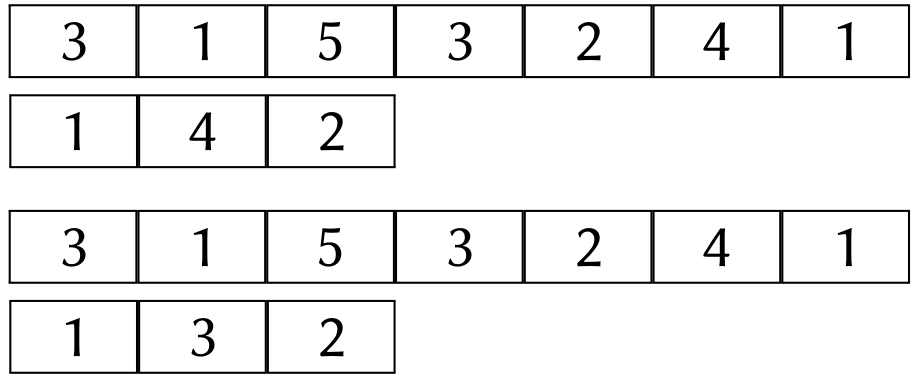
\includegraphics[width=0.4\textwidth]{lfd}
  \caption{Eingabe und Cache vor und nach Bearbeitung der ersten Anforderung. Es wird die \( 4 \) ersetzt, weil sie erst am weitesten in der Zukunft wieder benötigt wird}
\end{figure}

\subsection{Deterministisch --- bestenfalls \( k \)-kompetititv}

Die vier üblichen Algorithmen sind
\begin{itemize}
  \item fifo (\emph{first in first out}),
  \item lifo (\emph{last in first out}),
  \item lru (\emph{least recently used}),
  \item lfu (\emph{least frquently used}).
\end{itemize}

lifo und lfu sind nicht kompetitiv, lru und fifo sind \( k \)-kompetititv. In der Praxis wird üblicherweise lru verwendet.

Es gilt folgender Satz:

\begin{theorem}
  Jeder deterministische Online-Algorithmus für das Seitenwechselproblem mit Cachegröße \( k \) hat einen Wettbewerbsfaktor \( c \geq k \). \( k \) ist also eine untere Schranke für den Wettbewerbsfaktor.
\end{theorem}

\subsection{Deterministisch: lru ist \( k \)-kompetitiv}

Wir können zeigen, dass lru \( k \)-kompetititv ist.

\subsection{Resource Augmentation}

Wir betrachten das \( (h,k) \)-Seitenwechselproblem: hier wird der Online-Algorithmus \( \text{alg}_k \) mit der Cachegröße \( k \) mit \( \text{lfd}_h \) mit Cachegröße \( h < k \) verglichen.

Wir benötigen folgende Definition:

\begin{definition}
  Ein Online-Algorithmus heißt \term{konservativ}\index{Online-Algorithmus!konservativ}, falls er bei Andorderungsfolgen mit höchstens \( k \) verschiedenen Seiten höchstens \( k \) Cache-Misses hat.

  Beispiele hierfür sind lru und fifo.
\end{definition}

Es gilt:
\begin{equation*}
  \text{Jeder konservative Online-Algorithmus ist } \frac{k}{k-h+1} \text{-kompetitiv.}
\end{equation*}

\subsection{Randomisiert: randMark ist \( 2H_k \)-kompetititv}

Bei einem randomisierten Online-Algorithmus zur Speicherverwaltung ist die Zahl der Cache-Misses eine \emph{Zufallsvariable}
\begin{equation*}
  f_R(r_1,\dots,r_n)\text{.}
\end{equation*}

Hier sind gegebenenfalls andere Sichtweisen auf \( c \)-kompetitivität sinnvoll.

Zur Analyse verwenden wir sogenannte \term{Widersacher}\index{Widersacher}. Diese bekommen als Eingabe die gewünschte Länge \( n \) und \( R \) und erzeugen eine ``schlimme'' Anforderungsfolge der Länge \( n \). Diese müssen sie aber auch selbst verarbeiten.

Wir unterscheiden folgende Widersachertypen:

\begin{itemize}
  \item \term{unwissender Widersacher}\index{Widersacher!unwissend} \( W \) (\emph{oblivious adversary}): kein Wissen über erzeugte Zufallsbits, erzeugt für \( (R,n) \) immer gleiches \( (r_1,\dots,r_n) \).
  \item \term{adaptiver Widersacher}\index{Widersacher!adaptiv} \( W' \) (\emph{adaptive adversary}): arbeitet gegen eine konkrete Abarbeitung von \( R \), kennt die von \( R \) bei der Abarbeitung von \( (r_1,\dots,r_i) \) erzeugten Zufallsbits und folglich auch immer den aktuellen Cache-Zustand von \( R \).
\end{itemize}

Wir werden im Folgenden nur unwissende Widersacher analysieren und vergleichen sie mit \( \text{opt}(r_1,\dots,r_n) \).

\begin{definition}
  \( R \) ist \( c \)-kompetitiv gegen unwissende Widersacher, wenn es ein von \( n \) unabhängiges \( b \) gibt, sodass für jede Anforderungsfolge \( (r_1,\dots,r_n ) \) gilt:
  \begin{equation*}
    \textbf{E}[f_R(r_1,\dots,r_n)]-c*\text{opt}(r_1,\dots,r_n) \leq b\text{.}
  \end{equation*}
\end{definition}

Wir betrachten nun den randMark-Algorithmus.\footnote{Fiat et el., 1991}

\begin{pseudocode}
  \( \left\langle \text{Cache: cache}[i]\text{, Markierungsbits mark}[i], 1 \leq i \leq k \right\rangle \) \\
  \textbf{for} \( i \coloneqq 1 \) \textbf{to} \( k \) \textbf{do} mark\( [i] \coloneqq 0 \) \enskip \textcolor{gray}{// alle Markierungen auf \( 0 \)} \\
  \textbf{while} \( \exists \) weitere Anforderungen \textbf{do} \\
  \phantom{\enskip} \( r \coloneqq \) nächste Anforderung \\
  \phantom{\enskip} \textbf{if} \( \text{memory}[r] \not \in \) cache \textbf{then} \\
  \phantom{\enskip} \phantom{\enskip} \textbf{if} \( \forall \text{mark}[i] \equiv 1 \) \textbf{then} \( \forall \text{mark}[i] \coloneqq 0 \) \enskip \textcolor{gray}{// alles \( 1 \leadsto \) neue Phase \( \leadsto \) alles \( 0 \)} \\
  \phantom{\enskip} \phantom{\enskip} \( i \coloneqq \) zufälliges \( j \) mit \( \text{mark}[j] \equiv 0 \) \\
  \phantom{\enskip} \phantom{\enskip} \( \text{cache}[i] \coloneqq \text{memory}[r] \) \\
  \phantom{\enskip} \textbf{else} \( i \coloneqq \) Index mit \( \text{cache}[i] \equiv \text{memory}[r] \) \\
  \( \text{mark}[i] \coloneqq 1 \)

\end{pseudocode}

Dieser Algorithmus ist \( 2H_k \)-kompetitiv gegen unwissende Widersacher.

\section{Auswahl von Experten}

Es gibt mehrere Runden mit folgender Struktur:
\begin{enumerate}
  \item Jeder von \( n \) Experten gibt zu einer Frage eine Ja/Nein-Empfehlung ab. Diese sind im Allgemeinen nicht richtig.
  \item Man trifft seine eigene Ja/Nein-Entscheidung zu derselben Fragestellung.
  \item Es wird mitgeteilt, welche Entscheidung richtig gewesen wäre.
\end{enumerate}

Ziel ist:
\begin{itemize}
  \item \textbf{Anforderung}: \( k \)-Tupel aus Ja/Nein-Empfehlungen der Experten
  \item \textbf{Antwort}: Eigene Ja/Nein-Entscheidung
  \item \textbf{Kosten}: Anzahl eigener Fehlentscheidungen
  \item \textbf{Ziel}: Die eigenen Kosten sollen möglichst nah an den Kosten der besten Experten liegen
\end{itemize}

Es ist leicht einzusehen, dass immer die Antwort des Experten zu wählen, der bisher am meisten korrekte Antworten produziert hat, schlecht ist --- man kann eine Expertenmenge derart konstruieren, dass diese Strategie immer irrt.

\subsection{Weighted Majority Algorithm}

Der \term{Weighted Majority Algorithm}\index{Weighted Majority Algorithm} weist zu Beginn jedem Experte \( i \) ein Gewicht \( w_i \coloneqq 1 \) zu.

In jeder Runde wird die eigene Entscheidung nun folgendermaßen konstruiert:
\begin{enumerate}
  \item Experten geben Empfehlungen \( x_i \in \left \{ \text{ja}, \text{nein} \right \} \)
  \item Eigene Entscheidung fällen:
  \begin{equation*}
    \begin{cases}
      \text{ja,} \quad &\text{falls } \sum_{i,x_i\equiv \text{ ja}}w_i \geq \sum_{i,x_i \equiv \text{nein }}w_i \\
      \text{nein,} \quad &\text{falls } \sum_{i,x_i\equiv \text{ ja}}w_i < \sum_{i,x_i \equiv \text{nein }}w_i
    \end{cases}
  \end{equation*}
  \item Expertengewichte anpassen:
  \begin{equation*}
    w_i^{t+1} = \begin{cases}
      w_i^t\text{,} \quad &\text{falls \( x_i \) richtig war} \\
      \frac{w_i^t}{2}\text{,} \quad &\text{falls \( x_i \) falsch war}
    \end{cases}
  \end{equation*}
\end{enumerate}

wma ist \( \frac{1}{\log_2 (4/3)} \)-kompetitiv. Genauer:
\begin{equation*}
  \text{wma}(\sigma) \leq \frac{1}{\log_2 (4/3)}(\text{optExpert}(\sigma) + \log_2 k)\text{.}
\end{equation*}

\subsection{Verallgemeinerung}

Wir betrachten nun nicht mehr nur den Fall, dass Antworten richtig oder falsch sein können, sondern gewichten sie mit Faktoren zwischen \( 0 \) und \( 1 \). In der \( t \)-ten Runde läuft ab:

\begin{enumerate}
  \item \textbf{Experten}: geben Empfehlungen \( x_1, \dots, x_k \)
  \item Eigene Wahl der Empfehlung
  \item Mitteilung, welche Entscheidung richtig gewesen wäre
  \item Beurteilung der Empfehlungen durch ``Noten'' \( c_i^t \in [0,1] \)
  \item \textbf{Kosten}: Note der gewählten Empfehlung
\end{enumerate}

Wir verwenden hierfür einen randomisierten Algorithmus \( \text{randWMA}_\epsilon \):
\begin{itemize}
  \item Initial:
  \begin{itemize}
    \item Es sei \( \epsilon \in (0,\tfrac{1}{2}) \)
    \item Experte \( i \) hat Gewicht \( w_i \)
    \item alle \( w_i \coloneqq 1 \)
  \end{itemize}
  \item In jeder Runde \( t \):
  \begin{enumerate}
    \item wähle Empfehlung von Experte \( i \) mit Wahrscheinlichkeit
    \begin{equation*}
      p_i = \frac{w_i}{\sum_1^k w_i}
    \end{equation*}
    \item Benotung
    \item setze jedes \( w_i \coloneqq w_i(1-\epsilon c_i^t) \)
  \end{enumerate}
\end{itemize}

Ist \( k \) die Anzahl der Experten und \( 0 < \epsilon < \frac{1}{2} \) und \( \text{randWMA}_\epsilon \) nach einer Anzahl an Runden Gesamtkosten von \( K \) hat und die besten Experten Empfehlungen mit (minimalen) Gesamtkosten \( K_\text{opt} \) gegeben haben, so ist
\begin{equation*}
  K \leq (1+\epsilon)*K_\text{opt} + \frac{\ln n}{\epsilon}\text{.}
\end{equation*}